\section{Анализ подходов к решению проблемы}
\label{sec:analysis}

\subsection{Анализ предметной области}
Область медицины охватывает широкий спектр дисциплин, включая здравоохранение, диагностику, лечение и профилактику заболеваний. Среди множества проблем в этой области особенно актуальной является необходимость эффективного управления медицинской информацией. С ростом объема данных и сложности медицинских процессов возникает потребность в создании интеллектуальных систем, способных обрабатывать, анализировать и использовать эту информацию для поддержки принятия решений в медицинской практике.

Эта проблема актуальна по нескольким причинам:

\begin{itemize}
    \item Различные симптомы. Множество заболеваний человеческого организма проявляются через симптомы, которые могут быть схожи между собой, что затрудняет точную диагностику. Например, боль, слабость и повышенная температура могут быть признаками различных заболеваний, таких как грипп, пневмония или инфекционные заболевания желудочно-кишечного тракта. Это усложняет задачу врачей при определении конкретного заболевания и назначении соответствующего лечения.
    \item Недостаток данных. Для обучения моделей искусственного интеллекта необходимо большое количество данных, но доступ к таким данным ограничен из-за конфиденциальности и недостатка стандартизации.
    \item Сложность обработки изображений. Сложность обработки медицинских изображений также является проблемой, особенно в контексте анализа органов и тканей человеческого организма. Точная интерпретация медицинских снимков требует высокой экспертизы и может быть подвержена ошибкам, что усложняет автоматизацию этого процесса с помощью алгоритмов машинного обучения.
    \item Недостаточная точность алгоритмов. Некоторые алгоритмы могут быть недостаточно точными для диагностики сложных и разнообразных заболеваний человеческого организма, что ограничивает их применимость в клинической практике.
    \item Различие заболеваний. Болезни часто проявляются в различных формах и стадиях, что усложняет создание универсальных моделей для их диагностики. Таким образом, необходимо разработать подходы, которые учитывают эту вариабельность для более точной диагностики и прогнозирования.
\end{itemize}

Таким образом, хотя в области искусственного интеллекта в медицине достигнуты значительные успехи, точная диагностика заболеваний остается сложной задачей, требующей дальнейших исследований и улучшений в алгоритмах и технологиях.


\subsection{Анализ аналогов разрабатываемой системы}

\begin{enumerate}[label=\arabic*)]
  \item \textbf{ Woebot}(Рис. 1.1)[1]
  
Компания Woebot Labs запустила в эксплуатацию сервис, который они называют первым в мире автоматизированным чатом для помощи людям, страдающим от психиатрических заболеваний. 

Эта система рассматривается ее создателями как доступное, персонализированное и удобное лечение для миллионов людей, страдающих от психических заболеваний, связанных с изменениями настроения, такими как депрессия и тревожность. 

Чатбот использует методы когнитивно-поведенческой терапии, чтобы выслушать и дать совет любому, кто обратится к боту за помощью. С помощью разговора на обычном "человеческом"  языке приложение позволяет пользователю получить эмоциональную поддержку, которая ему нужна, и научиться практическим методам, позволяющим изменить ход мыслей о происходящих в его жизни явлениях. 

\begin{figure}[h]
    \centering
    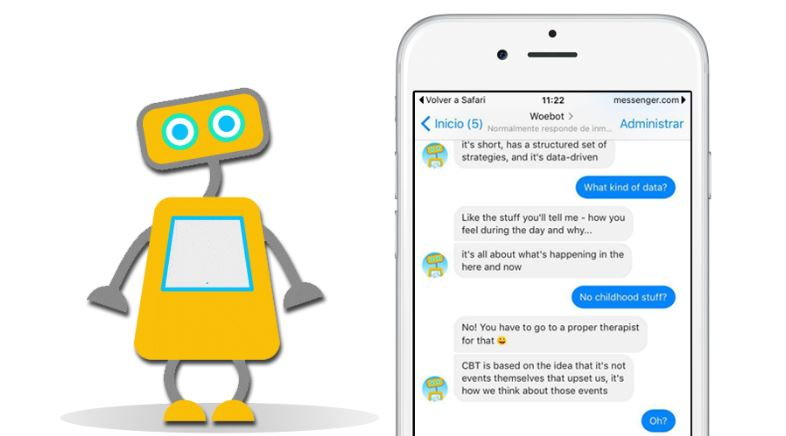
\includegraphics[width=1\textwidth]{sections/woebot.jpg}
    \caption{Пример использования помощника Woebot}
    \label{fig:example}
\end{figure}

\textbf{Преимущества:}
\begin{itemize}
    \item сайт предлагает широкий спектр информации о различных аспектах здоровья, включая симптомы, лечение и профилактику различных заболеваний, питание, физическую активность и т.д.;
    \item информация о заболеваниях, симптомах и лечении представлена в достаточной степени подробно;
    \item наличие статей и руководств, которые могут быть полезны для понимания различных аспектов здоровья и медицины;
    \item cайт имеет простой и удобный интерфейс, что делает его доступным для широкого круга пользователей;
    \item информация представлена в виде статей, списков симптомов, советов по лечению и т.д., что упрощает поиск нужной информации;
    \item наличие поисковой строки позволяет пользователям быстро находить интересующие их темы и статьи.
\end{itemize}
\textbf{Недостатки: }
\begin{itemize}
    \item cайт не предоставляет явной информации о своих источниках данных и контенте;
    \item в большинстве статей нет ссылок на научные исследования или медицинские источники, что может вызывать сомнения в достоверности представленной информации;
    \item отсутствие анонсированных авторов статей или специалистов, которые подтверждали бы их квалификацию, также может влиять на восприятие сайта как недостаточно достоверного источника медицинской информации.
\end{itemize}

В целом, сайт Woebot предоставляет обширную информацию о различных аспектах здоровья и медицины, что может быть полезным для пользователей, заинтересованных в самостоятельном изучении этих тем.

Однако отсутствие явной информации о источниках и недостаточная ссылочность на научные исследования может вызвать вопросы о достоверности представленной информации. Поэтому при использовании данного ресурса важно проявлять осторожность и проверять информацию в других источниках, особенно если речь идет о серьезных медицинских вопросах или лечении. Также недостатком данного помощника является то, что он расчитан на психологическую помощь, а консультации по вопросам заболеваний, например, мышечных тканей или легких путей он не способен проводить. 


  \item \textbf{HealthTap}(Рис. 1.2) [2]
  
HealthTap - это инновационная медицинская онлайн-платформа, предоставляющая широкий спектр медицинских консультаций
и услуг через виртуальный чат. Эта платформа была разработана для того, чтобы сделать медицинские консультации более доступными и удобными для пользователей, независимо от их местоположения.

Пользователи HealthTap могут получать квалифицированные медицинские советы и консультации от настоящих медицинских специалистов в режиме реального времени. Это позволяет пользователям получать экспертные мнения по широкому спектру медицинских вопросов, начиная от общих симптомов и заканчивая конкретными запросами.

\begin{figure}[h]
    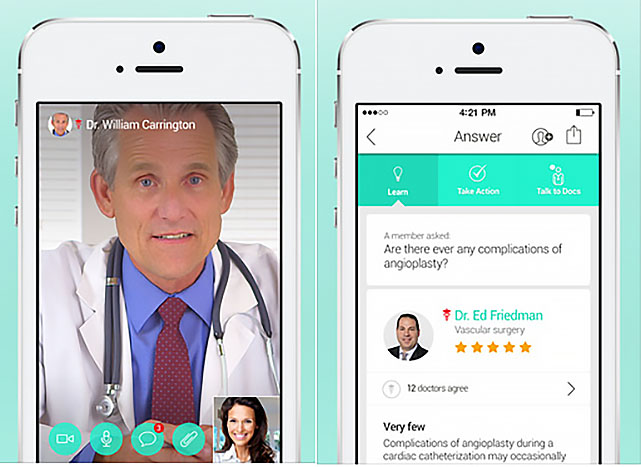
\includegraphics[width=1\textwidth]{sections/healthtap.jpg}
    \caption{Пример использования помощника HealthTap}
    \label{fig:example}
\end{figure}

\textbf{Преимущества:}
\begin{itemize}
    \item HealthTap предлагает обширный объем информации о здоровье и медицине, включая симптомы, диагностику, лечение различных заболеваний, советы по здоровому образу жизни и т. д..
    \item сайт содержит разнообразные статьи, ответы на вопросы пользователей, видеоинструкции, часто задаваемые вопросы и т. д., что делает его информативным и полезным ресурсом для пользователей, заинтересованных в здоровье.
    \item Конфиденциальность и безопасность данных. Защита конфиденциальности данных пользователей находится в приоритете, обеспечивая им уверенность в безопасности информации.
    \item Статьи и ответы на вопросы часто сопровождаются ссылками на научные исследования, клинические рекомендации и другие авторитетные источники, что способствует доверию к контенту.
    \item Сайт имеет простой и интуитивно понятный интерфейс, что облегчает поиск и чтение информации для пользователей.
    \item Наличие функции поиска позволяет пользователям быстро находить нужные им темы и статьи.
    \item HealthTap также предоставляет возможность задавать вопросы медицинским экспертам и получать консультации в режиме онлайн, что делает его полезным ресурсом для получения персонализированной медицинской информации.
\end{itemize}

\textbf{Недостатки:}
\begin{itemize}
    \item Платная услуга в большинстве случаев. Один из недостатков HealthTap заключается в том, что доступ к его услугам часто предполагает плату, что может ограничивать доступность для пользователей с ограниченными средствами.
    \item Не всегда доступно вне США. Географические ограничения могут сделать HealthTap менее доступным для пользователей за пределами Соединенных Штатов.
\end{itemize}

Сайт HealthTap представляет собой полезный и информативный ресурс о здоровье и медицине, который предлагает широкий спектр информации для пользователей.

Утверждение о том, что контент разрабатывается медицинскими специалистами и ссылки на научные исследования улучшают доверие к представленной информации.

Однако, как и в случае с любым другим медицинским ресурсом, важно проявлять осторожность и проверять информацию в других независимых источниках, особенно при решении серьезных медицинских вопросов.

  \item \textbf{ Ada Health}(Рис. 1.3)[3]

Платформа Ada, доступная через бесплатное приложение для смартфонов, проводит пользователей через серию вопросов о демографических характеристиках, основных параметрах здоровья и любых симптомах, которые они испытывают, а также о начале и тяжести этих симптомов. Затем приложение использует алгоритм искусственного интеллекта для сравнения данных, предоставленных пользователями, с обширной медицинской библиотекой Ada, чтобы составить список заболеваний, которые могут быть причиной симптомов.

Алгоритм был обучен специфике сотен медицинских заболеваний, что позволяет ему выявлять мельчайшие различия между симптомами и основными факторами здоровья, связанными с заболеваниями, которые могут проявляться схожим образом.

Разработчики утверждают, что в будущем Ada станет стандартным диагностическим инструментом для врачей. Это уже происходит - пользователи могут поделиться своей оценкой состояния здоровья со своим врачом или (в Великобритании) они могут проконсультироваться с квалифицированным терапевтом через функцию "Чат с врачом". Ada также станет гораздо более постоянным спутником здоровья, помогая пациентам и врачам разумно отслеживать данные о здоровье в течение длительного времени, чтобы обеспечить предиктивное и проактивное лечение.

\begin{figure}[h]
    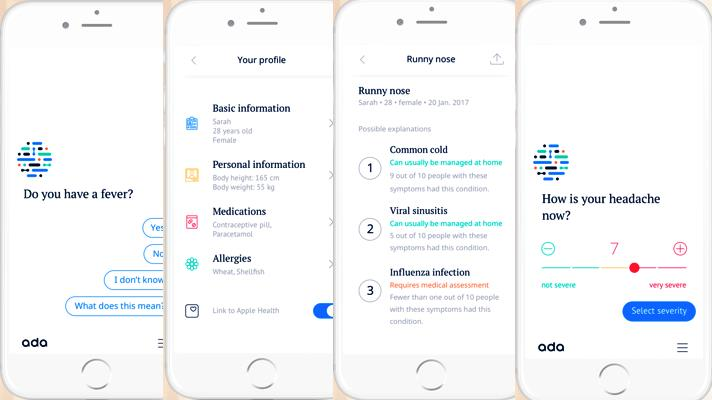
\includegraphics[width=1\textwidth]{sections/Ada Health TN.jpg}
    \caption{Пример использования помощника Ada Health}
    \label{fig:example}
\end{figure}

\textbf{Преимущества:}
\begin{itemize}
    \item Ada Health обеспечивает высокую точность диагнозов, основанных на симптомах и медицинских данных. Это позволяет пользователям получать надежные информацию о своем здоровье.
    \item Сайт также предоставляет инструмент для самодиагностики, позволяющий пользователям оценить свои симптомы и получить предварительные рекомендации по дальнейшим действиям.
    \item Возможность ввода симптомов и получения рекомендаций. Пользователи могут легко и подробно описывать свои симптомы, что делает систему доступной и интуитивно понятной.
    \item Интеграция с базой знаний и медицинскими данными.
    \item Сайт имеет простой и интуитивно понятный интерфейс, что облегчает навигацию и поиск информации для пользователей в базе знаний с актуальными медицинскими данными, что повышает информативность и надежность предоставляемой информации.
    \item Ada предлагает информацию о различных аспектах здоровья, включая симптомы, возможные причины, диагностику и лечение различных заболеваний.
    \item Ada утверждает, что его контент разрабатывается медицинскими экспертами и основан на актуальных клинических рекомендациях и научных исследованиях.
    \item Статьи и информация часто сопровождаются ссылками на медицинские источники и авторитетные медицинские организации, что способствует доверию к представленной информации.
    \item Функция самодиагностики позволяет пользователям оценить свои симптомы и получить предварительные рекомендации по медицинской помощи.
\end{itemize}

\textbf{Недостатки:}
\begin{itemize}
    \item Ограничения в медицинских консультациях. Ada Health не заменяет полноценных врачей и может быть ограничена в предоставлении консультаций в случае серьезных заболеваний или нестандартных ситуаций
\end{itemize}


Сайт Ada Health представляет собой полезный и информативный ресурс о здоровье и медицине, который предлагает широкий спектр информации для пользователей.
Утверждение о том, что контент разрабатывается медицинскими экспертами, и ссылки на научные исследования улучшают доверие к представленной информации.

\end{enumerate}

После рассмотрения всех аналогов и выявления их достоинств и недостатков, можно сделать вывод о том, что ни один из аналогов полностью не удовлетворяет всем требованиям, которые должны быть в нашей медицинской системе.

 Исходя из анализа аналогов, можно выделить следующие основные требования к медицинской системе:

\begin{enumerate}[label=\arabic*)]
     \item Наполняемость базы знаний (БЗ):
        \begin{itemize}
            \item система должна иметь обширную и достоверную базу знаний о различных аспектах здоровья и медицины, включая симптомы, диагностику, лечение и профилактику различных заболеваний;
            \item информация должна быть представлена в понятной и доступной форме, чтобы пользователи могли легко находить нужную информацию.
        \end{itemize}
    \item Достоверность источников:
        \begin{itemize}
            \item система должна основываться на достоверных источниках данных, таких как клинические рекомендации, научные исследования и медицинские практики;
            \item информация должна быть проверена медицинскими экспертами и специалистами, чтобы обеспечить высокую точность и достоверность.
        \end{itemize}
    \item Доступ к информации:
        \begin{itemize}
            \item система должна предоставлять удобный и интуитивно понятный интерфейс для пользователя, облегчающий поиск и чтение медицинской информации;
            \item наличие функции поиска и катетеризации информации позволит пользователям быстро находить нужные им темы и статьи;
            \item возможность получения персонализированных консультаций от медицинских экспертов или использования инструментов самодиагностики может повысить ценность системы для пользователей.
        \end{itemize}
    \item Безопасность данных:
        \begin{itemize}
            \item Cистема должна обеспечивать конфиденциальность и безопасность медицинских данных пользователей, соблюдая соответствующие стандарты и законодательство о защите данных.
        \end{itemize}
 \end{enumerate}
 
\subsection{Анализ подходов к разработке}

Для разработки медицинского ассистента нужно создать базу знаний, для реализации которой могут использоваться:

\begin{itemize}
    \item Технология OSTIS
    \item Semantic Web
\end{itemize} 

\subsubsection{Технология OSTIS}

В рамках усовершенствования процесса диагностики с предварительным анализом, на последующих этапах разработки предусмотрено внедрение обширной базы знаний, охватывающей разнообразные медицинские темы. Это нововведение будет способствовать повышению точности диагностических процедур, предоставлению индивидуализированных советов и поддержке пациентов.
Технология OSTIS была выбрана для создания этой базы знаний благодаря её способности к гибкой адаптации под различные задачи и области знаний. OSTIS эффективно справляется с анализом неоднозначной и неполной информации, что делает его эффективным инструментом для моделирования сложных сценариев. Это делает OSTIS ценным инструментом для моделирования сложных сценариев. Для внешнего представления SC-кода был выбран SCg, как наиболее подходящий для разработки.

Преимущества технологии OSTIS:
\begin{itemize}
	\item имеет строгую теоретико-множественную трактовку и не привязаны к конкретной прикладной области;
	\item имеет возможность представления отношений любой арности;
	\item отношения представляются в виде узлов семантической сети, что позволяет характеризовать их свойства;
	\item экземпляры отношений выделяются как отдельные узлы семантической сети, что дает возможность характеризовать каждый экземпляр отношения уникальным образом;
	\item в алфавите ключевых узлов и дуг имеются элементы для описания нечетких, негативных и нестационарных объектов.
\end{itemize}

Ключевым элементом интеллектуальных систем OSTIS являются решатели задач — специализированные компоненты, которые дают системе возможность обрабатывать запросы пользователей. Эти решатели задач используют данные из базы знаний для анализа, обработки и предоставления ответов на вопросы, заданные пользователями в свободной форме. Они функционируют на основе знаний, представленных в SC-коде, и позволяют автоматизировать решение прикладных задач в различных областях.


\subsection{Анализ подходов к управлению проектом}

Также для обеспечения эффективного выполнения проекта необходимо воспользоваться одной из методологий управления проектом. Выберем наиболее подходящую из:

\begin{itemize}
    \item Waterfall (Водопад)
    \item Метод критического пути
    \item Agile
    \item Scrum
\end{itemize}
\subsubsection{Agile}

 Методология управления проектами Agile является одним из наиболее распространённых подходов к управлению проектами. Однако, по сути, Agile — принцип управления проектами. 

В основе Agile лежат следующие принципы:

\begin{itemize}
    \item совместная работа
    \item скорость и эффективность
    \item итеративность и ориентация на данные
    \item личность важнее процессов
\end{itemize}

Когда дело доходит до внедрения Agile, команды часто выбирают определённую методологию, которую они будут использовать наряду с принципами Agile. Это может быть Scrum, Kanban, экстремальное программирование, Crystal или даже Scrumban. Делается это потому, что использование методологии Agile вместе с более подробно сформулированным подходом позволяет сформировать законченную философию управления проектом и практический план для достижения отличных результатов.

\textbf{Кому подойдёт.} Систему Agile может использовать практически любая команда, потому что в её основе лежат довольно универсальные принципы. Самое сложное здесь — решить, какую методологию использовать совместно с этим подходом.

\subsubsection{Waterfall (Водопад)}

Каскадная модель управления, также известная как «водопад», довольно популярна. «Водопад» — это настоящая методология с очень чёткими правилами. Каскадная методология, также известная как цикл разработки программного обеспечения (ЦРПО) представляет собой линейный процесс, в котором работа ниспадает каскадом (как водопад) и организована в последовательном порядке.

При использовании этого подхода все рабочие задачи связываются друг с другом зависимостями. Это означает, что для того, чтобы начать работу над задачей, должна быть выполнена предшествующая ей задача. Благодаря этому работа идёт по плану, а также обеспечивается чёткий обмен информацией в течение всего процесса.

Хотя некоторые современные организации считают данный подход устаревшим, эта методология отлично подходит для создания предсказуемого и хорошо продуманного плана проекта. 

\begin{figure}[H]
    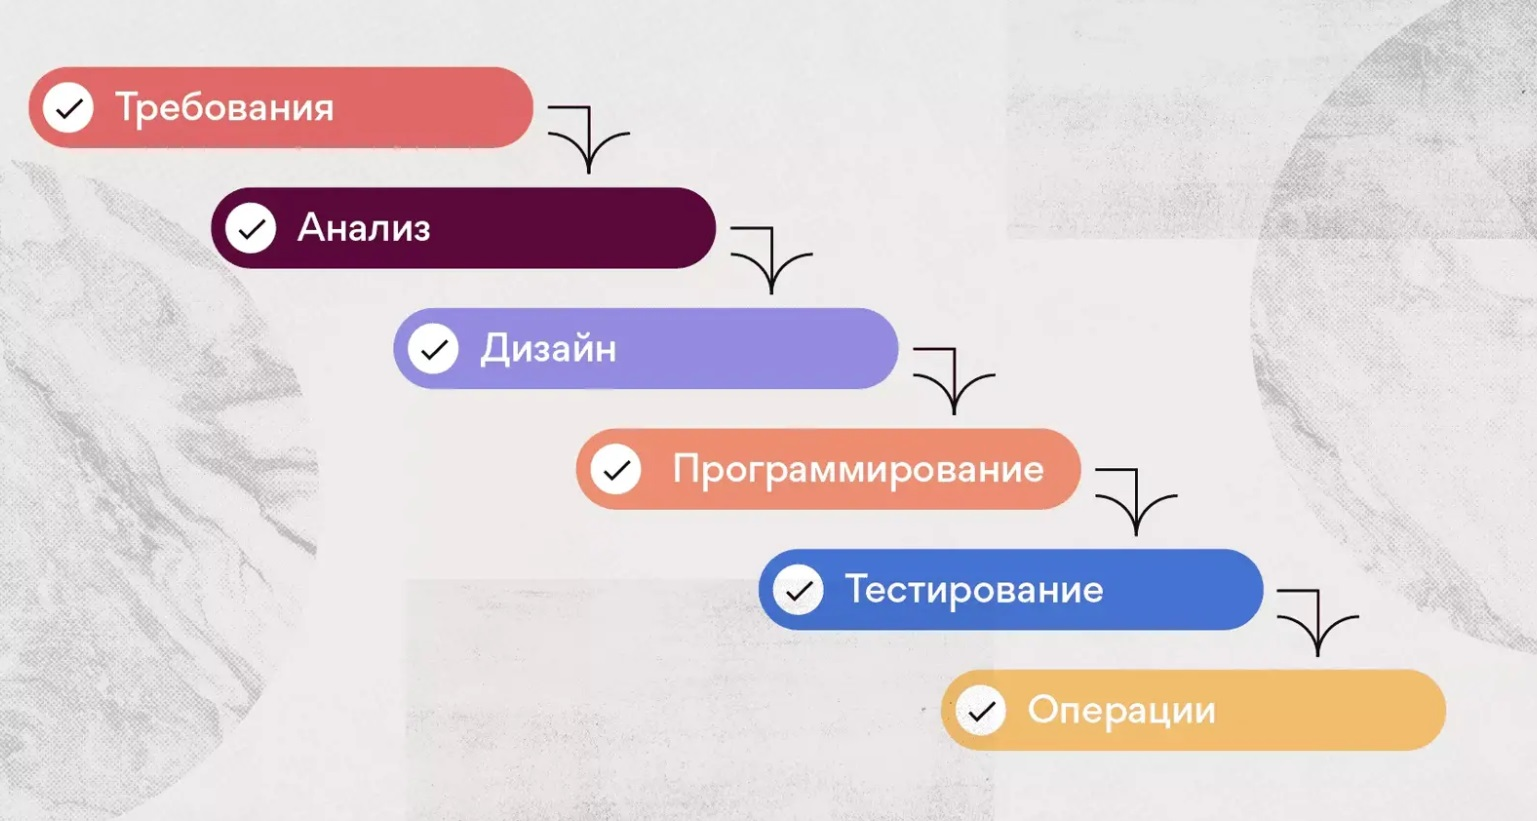
\includegraphics[width=1\textwidth]{sections/waterfall.jpg}
    \caption{Пример модели управления Waterfall}
    \label{fig:example}
\end{figure}

\textbf{Кому подойдёт.} Поскольку каскадная методология управления является очень подробной, она хорошо подходит для работы над крупными проектами с множеством заинтересованных сторон. Эта модель обеспечивает наличие чёткой информации о необходимых действиях в течение всего проекта и зависимостей, позволяющих отследить работу, которую следует выполнить для достижения целей. 

\subsubsection{Метод критического пути}

Метод критического пути применяется для определения критически важных задач в проекте и планирования работы над ними. Сюда входит создание зависимостей между задачами, отслеживание целей проекта и хода работ над ним, определение приоритета результатов и управление сроками — все это очень похоже на структуру разбивки работ.

Цель этой методологии состоит в надлежащем управлении успешными проектами в масштабе так, чтобы вехи и ожидаемые результаты были размечены правильно.

\textbf{Кому подойдёт.} Метод критического пути лучше всего подходит для небольших и средних проектов и команд. Связано это с тем, что в крупных проектах множество ожидаемых результатов и заинтересованных сторон, а метод критического пути не предназначен для сложных проектов. 

\subsubsection{Scrum} 

 Методология Scrum предусматривает использование коротких «спринтов», из которых формируется цикл проекта. Эти промежутки длятся от одной до двух недель и рассчитаны на команды в составе не более 10 человек. Это основное отличие от каскадной методологии, где отдельные задачи связываются друг с другом зависимостями.

У Scrum много уникальных особенностей, одной из которых является наличие мастера Scrum или, другими словами, руководителя проекта, который проводит ежедневные Scrum-совещания, демонстрации, спринты и ретроспективы после окончания спринтов. Все эти встречи нужны для общения ключевых участников проекта и своевременного выполнения задач.

Несмотря на то, что технически Scrum является самостоятельной методологией управления проектами, её часто ассоциируют с системой Agile. Связано это с тем, что два этих подхода объединены общими принципами, в том числе принципом важности совместной работы и тем, что личность ценится выше процессов.

\textbf{Кому подойдёт.} Командам, применяющим подход Agile, также следует прибегнуть к методологии Scrum, или, по крайней мере, попробовать её в действии. Так как спринты проводятся для небольших команд, этот подход работает как для небольших, так и для крупных коллективов. 

\subsection{Вывод}

Проведенный анализ позволяет сделать вывод об актуальности и важности разработки и внедрения системы медицинского ассистента. Такие системы становятся все более необходимыми в нашем цифровом мире, где доступ к информации и консультациям в области здоровья и медицины играют ключевую роль для обеспечения качественного и своевременного медицинского обслуживания. Медицинские ассистенты предоставляют пользователю доступ к обширной базе знаний, консультациям медицинских экспертов и инструментам самодиагностики, что повышает уровень информированности и помогает в принятии обоснованных решений по вопросам здоровья.

Исходя из проведенного анализа можно сделать заключение о необходимости следующих требований к базе знаний системы медицинского ассистента:

\begin{itemize}
    \item Обширность и достоверность информации. База знаний должна содержать подробную и актуальную информацию о различных аспектах здоровья и медицины, проверенную медицинскими экспертами и основанную на научных исследованиях и клинических рекомендациях.
    \item Удобство доступа и навигации. Пользователям должен быть предоставлен удобный интерфейс для поиска и чтения медицинской информации, а также функции категоризации и фильтрации контента для быстрого доступа к нужным темам.
    \item Поддержка персонализированных консультаций. База знаний должна поддерживать возможность получения персонализированных консультаций от медицинских экспертов, а также предоставления инструментов самодиагностики для пользователей.
\end{itemize}

Также на основе проведенного анализа можно сделать заключение о необходимости следующих требований к разрабатываемым решателям задач:

\begin{enumerate}[label=\arabic*)]
    \item Достоверность информации. Решатель задач должен реализовывать свою работу на основе разработанной базы знаний, содержащей подробную и актуальную информацию о различных аспектах здоровья и медицины, проверенную медицинскими экспертами и основанную на научных исследованиях и клинических рекомендациях, а также предоставлять на ее основе достоверную информацию о результате работы.
    \item Удобство доступа. Пользователям должен быть предоставлен удобный интерфейс для вызова и отслеживания результатов работы вызываемых решателей задач в интеллектуальной системе.
    \item Критический подход к интерпретации данных. Пользователю должна быть предоставлена информация о необходимости прохождения дальнейшей диагностики у соответствующего профильного специалиста в связи с отсутствием возможности поставить в достаточной степени достоверный результат по результатам самодиагностики.
\end{enumerate}

Для разработки системы была выбрана технология OSTIS и выделены её преимущества. Эта технология поможет улучшить функциональность и эффективность медицинского ассистента, обеспечивая высокую точность диагностики, скорость обработки данных, автоматизацию процессов, адаптивность к изменениям и безопасность информации.

Наиболее предпочтительным для разработки и реализации данного проекта его участниками был выбран подход к управлению 'Метод критического пути', включающий в себя принципы Agile и элементы Scrum, такие как наличие руководителя проекта и ретроспективы по результатам окончания спринта. Таким образом, будет достигнута возможность планировать совместную разработку и реализацию проекта, а также проводить своевременные корректировки и анализ проделанной работы, где каждый из участников будет выполнять поставленные задачи.

Также для обеспечения работоспособности и возможности реализации работы некоторых из решателей задач, в частности, направленных на диагностику заболеваний по результатам анализов, необходимо актуализировать и расширить ранее разработанную базу знаний в области медицинских анализов.













